% ═════════════════════════════════════════════════════════════════════════════
% CHAPTER 3: État de l'Art (State of the Art)
% Restructured for proper thesis hierarchy
% Original content preserved between markers - DO NOT EDIT
% ═════════════════════════════════════════════════════════════════════════════

\chapter{State of the Art and Technical Foundations}
\label{chap:state-of-art}

% ═════════════════════════════════════════════════════════════════════════════
\section{\textcolor[HTML]{0066CC}{Artificial Intelligence}}
\label{sec:ai-basics}
% ═════════════════════════════════════════════════════════════════════════════

\subsection*{\textcolor[HTML]{003D99}{Overview and Historical Development}}

Artificial intelligence is a field of computer science which deals with the designing of intelligent systems, capable of performing human like tasks using algorithms which are developed and built upon in a computational framework. Systems with high enough capability can be regarded as intelligent to do human traditional tasks such as natural language understanding.
\begin{figure}[!htbp]
  \centering
  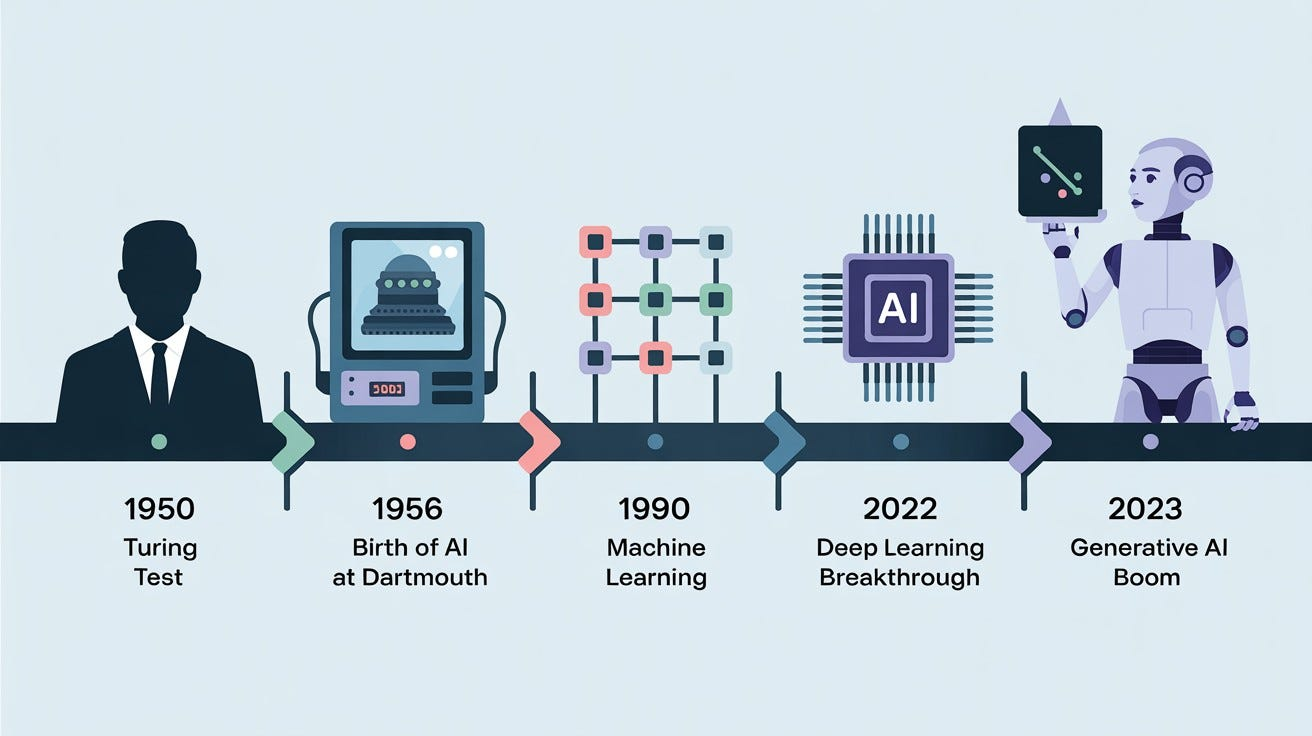
\includegraphics[width=0.75\textwidth]{images_pfe/history AI.jpg}
  \caption{Historical development of Artificial Intelligence.}
  \label{fig:history_ai}
\end{figure}
The specific term of artificial intelligence was first uttered as far back as 1956 by John McCarthy in his proposal for the Dartmouth Summer Research Project on Artificial Intelligence. AI has since progressed in phases, beginning with the symbolic and then experiencing a fall in popularity called an AI winter. Modern techniques have evolved in the form of deep learning, inspired by artificial neural networks.

\subsection*{\textcolor[HTML]{003D99}{Key Methodologies}}

To better understand this discipline, it is useful to distinguish several key authorities:

\noindent\textbf{Symbolic approaches:} In this domain, symbolic methodologies have a special advantage because of their ability to handle explicit knowledge. They are used for formalizing the rules of dialogue of a language (for example, in systems that have a natural language interface), and for implementing rule-based systems.

\noindent\textbf{Machine learning} allowing computers to acquire knowledge automatically from data and is also an important element to customize the Chatbots based on the users.

\noindent\textbf{The statistical approach} is more linked to the underlying theory because it attempts to make the uncertainty explicit by using probabilistic theory and is a statistical implications. It does this by representing uncertainty through probabilistic and statistical methods such as probability theory and Bayesian estimation.

\noindent\textbf{Artificial neural networks,} which form the basis of deep learning. One way to motivate neural networks is by the fact that the mechanisms involved are biologically analogous to human brain (Hertz et al., 1991, Domingos 2012). The methods developed are powerful for generate text and fused multimedia data.

\subsection*{\textcolor[HTML]{003D99}{Current Applications and Impact}}

In recent times, the uses of AI are vast and expanding. Speech recognition, computer vision, and recommenders systems are just some examples where AI are used widely. The combination of big data, greater processing power, and newalgorithmsare among the important reasons why artificial intelligence is getting popular recently.
\begin{figure}[!htbp]
  \centering
  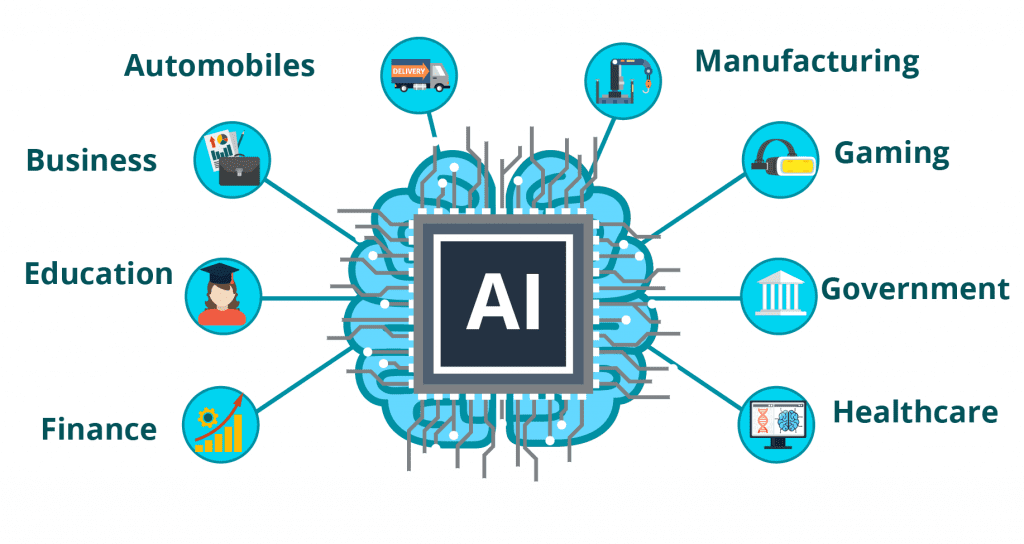
\includegraphics[width=0.75\textwidth]{images_pfe/AI use.png}
  \caption{Current applications and impact of Artificial Intelligence.}
  \label{fig:ai_uses}
\end{figure}
\FloatBarrier

% ═════════════════════════════════════════════════════════════════════════════
\section{\textcolor[HTML]{0066CC}{Generative Artificial Intelligence}}
\label{sec:generative-ai}
% ═════════════════════════════════════════════════════════════════════════════

\subsection*{\textcolor[HTML]{003D99}{Definition and Core Concepts}}

Generative AI employs all methods and models that generate original content text, images, music, audio, video, or other digital media in response to a prompt or to learn an AI lean an attention-based mechanism used primarily to generate the output a specific task, such as predicting a future outcome, categorizing things or clarifying features. AI. The generative model differs from other IM models in that it needs to learn the overall distribution of the training data rather than just learning to classify patterns or characteristics and can use this knowledge to create entirely new outputs that would have never exist on its own.

\begin{figure}[!htbp]
  \centering
  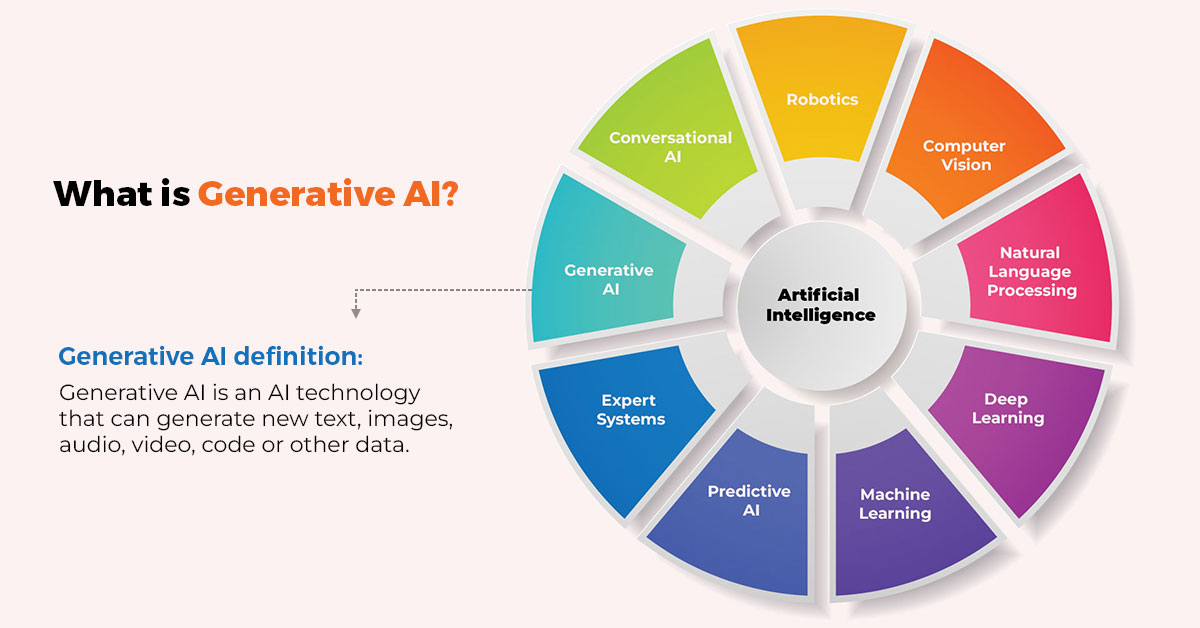
\includegraphics[width=0.75\textwidth]{images_pfe/GenAI.jpg}
  \caption{Concept of Generative Artificial Intelligence.}
  \label{fig:concept_generative_ai}
\end{figure}

\subsection*{\textcolor[HTML]{003D99}{Foundation Models: Concept and Role}}
\label{subsec:foundation-models}
The core of many different large scale or multimodal generative AI is a foundation model, typically either a large language model based chatbot like OpenAI's ChatGPT, Anthropic's Claude, or multimodal generator models for images, text-to-image generators for example. As given a foundation model is a model trained on broad data at scale to solve many tasks (using self-supervised learning and can be adapted to a wide range of downstream tasks.

\begin{figure}[!htbp]
  \centering
  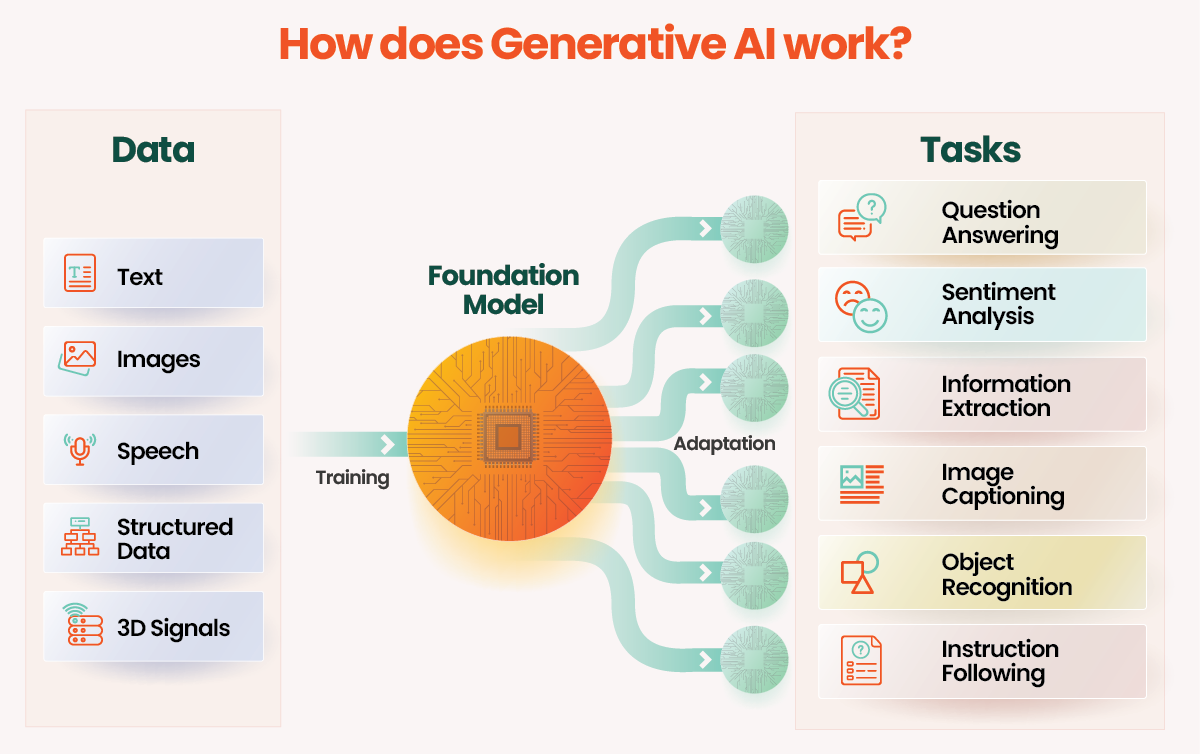
\includegraphics[width=0.75\textwidth]{images_pfe/foundation model.png}
  \caption{Concept of Foundation Models in Generative AI.}
  \label{fig:foundation_model}
\end{figure}

Self-supervised pretraining (SSP) for vision-language representations. In practice, large-scale pretraining, often referred to as pretraining, trains a model to produce representations for a wide variety of tasks based on diverse datasets, often using self-supervised or self-supervised learning methods.

Another important property of foundation models is that it is possible to adapt the same pre-trained model to multiple tasks without having to retrain from scratch each time; this can be accomplished by fine-tuning the model, instruction prompting, or through other techniques.

Furthermore, training foundational models requires significant amounts of resources and compute.

Another key reason for flexibility comes from the use of transfer learning, an area in which the foundation excel. The broad distribution of the knowledge used in pretraining is the core factor, because knowledge learned is often helpful for a variety of related downstream tasks.

\subsection*{\textcolor[HTML]{003D99}{Typology of Foundation Models}}
\label{subsec:foundation-typology}

There are a few main types of foundation models to consider: models designed for specific modalities (e.g., text, images, audio, video); models focused on specific capabilities (e.g., reasoning or generative). Foundation models are, in our framing, characterized by the usage of broad data at scale, such that they can adapt to many downstream tasks generic and broadly, often through selfsupervision.

\vspace{0.1cm}

\noindent\textcolor[HTML]{0066CC}{\textbf{Foundation Model Families and Their Applications:}}

\begin{table}[h!]
\centering
\caption{Typology of Foundation Models in Artificial Intelligence: Families, Descriptions, and Representative Examples}
\label{tab:foundation-typology}
\footnotesize
\setlength{\tabcolsep}{4pt}
\renewcommand{\arraystretch}{1.3}
\begin{tabularx}{\textwidth}{|>{\raggedright\arraybackslash}p{2.5cm}|>{\raggedright\arraybackslash}X|>{\raggedright\arraybackslash}X|}
\hline
\rowcolor[HTML]{0066CC}\color{white}\textbf{Foundation Model Family} & \color{white}\textbf{Description} & \color{white}\textbf{Representative Examples and Typical Use Cases} \\
\hline
\textcolor[HTML]{003366}{\textbf{Computer Vision Foundation Models}} & Models designed to analyze, interpret, and generate visual content (images and, in some cases, video) within a unified framework. & Florence: image description, visual question answering, object recognition, real-time video integration. \\
\hline
\textcolor[HTML]{003366}{\textbf{Unified Multimodal Foundation Models}} & Models capable of processing multiple input types (text, images, audio, video) and learning complex cross‑modal semantic relationships for richer contextual understanding. & GPT-4o (OpenAI), Gemini 2.0 (Google DeepMind), LLaMA 3.2 (Meta): advanced multimodal generation and understanding. \\
\hline
\textcolor[HTML]{003366}{\textbf{Large Language Models (LLMs) based on Transformers}} & Deep models built on Transformer architectures, specialized in understanding and generating natural language with strong contextual coherence. & Creation of ultra-realistic images, generation of synthetic data, enhancement of astronomical images, controlled deepfakes. \\
\hline
\textcolor[HTML]{003366}{\textbf{Generative Adversarial Networks (GANs)}} & Architectures composed of two neural networks trained in competition (generator vs. discriminator) to produce samples resembling training data. & GPT-3.5, GPT-4, Claude 3.5 (Anthropic), Mistral Large (open source), Grok (xAI): conversation, coding, complex reasoning. \\
\hline
\end{tabularx}
\end{table}

\FloatBarrier

\vspace{0.3cm}

In conclusion, these new models is a giant leap in AI field because they are capable of tackling vast number of unlabeled data and different task type, also they leverage multiple architecture styles, particularly transformers. Also, self-supervised learning seems to be a highly effective strategy for model training.\\
In order to perform this kind of task,  several computer vision models exist such as:  \textbf{Florence} (that understands the content of pictures),  \textbf{multimodal models (GPT-4,  Gemini 2.0)} that mix different types of data for their predictions,  \textbf{GANs (Good Automatic Networks)} which generate similar images, or \textbf{LLM (Long Large Models)} such as GPT-4 or Claude 3.5 which can predict natural text.\\

\subsection*{\textcolor[HTML]{003D99}{Traditional AI vs. Generative AI}}
\label{subsec:generative-vs-traditional}

GenAI systems are qualitatively different from earlier forms of \textbf{AI (e.g., Expert Systems, Machine Learning Classification/Regression models, etc.)}. Unlike prior applications of AI, which primarily made predictions on structured data and produced predictions within that structured domain (numbers, categories), GenAI is designed to produce new forms of unstructured data such as \textbf{text, images, audio, etc.} This new capability has been enabled by a particular architecture called the foundation model, particularly based on self-supervised learning using Transformer models trained on vast, diverse data.
\vspace{0.3cm}

\noindent\textcolor[HTML]{0066CC}{\textbf{Comparative Analysis: Traditional AI vs. Generative AI}}
\begin{table}[!htbp]
\centering
\caption{Comparison between Traditional AI and Generative AI}
\label{tab:traditional-vs-generative-ai}
\small
\begin{tabularx}{\textwidth}{|>{\raggedright\arraybackslash}p{2.5cm}|>{\raggedright\arraybackslash}X|>{\raggedright\arraybackslash}X|}
\hline
\rowcolor[HTML]{0066CC}\color{white}\textbf{Aspect} & \color{white}\textbf{Traditional AI} & \color{white}\textbf{Generative AI} \\
\hline
\textcolor[HTML]{003366}{\textbf{Type of content}} & Structured (tables, databases) & Unstructured (text, images, audio, video) \\
\hline
\textcolor[HTML]{003366}{\textbf{Models used}} & Task-specific models, often supervised & Foundation models (Transformers, LLMs) \\
\hline
\textcolor[HTML]{003366}{\textbf{Learning}} & Specific, labeled data & Large unlabeled datasets, self-supervised learning \\
\hline
\textcolor[HTML]{003366}{\textbf{Capabilities}} & Classification, prediction & Content generation, classification, prediction \\
\hline
\textcolor[HTML]{003366}{\textbf{Versatility}} & Limited to a specific task & Versatile, multi-task \\
\hline
\textcolor[HTML]{003366}{\textbf{Application examples}} & Object recognition, fraud detection & ChatGPT, DALL·E 2, Stable Diffusion, Bard \\
\hline
\textcolor[HTML]{003366}{\textbf{Limitations}} & High performance on a single task & Risk of hallucinations, lack of explainability \\
\hline
\end{tabularx}
\end{table}

\FloatBarrier

By comparison,  most of the \textbf{traditional AI} is narrowly defined in purpose,  and will typically perform analysis, classification, or prediction based on structured or semi-structured information.  The core advantage is its higher level of accuracy, since it is trained to perform a very specific function on a specific data set.

On one hand,  foundation models seem incredibly flexible, not only do they excel at most specific downstream tasks,  the same model appears adaptable to new tasks and domains, and capable of generating much more diverse and unexpected outputs.

On the other hand,  we note that generative AI do have some major drawbacks.  Firstly,  \textbf{hallucination phenomenon} which generates inaccurate, fake responses; lack of explainability, where the outputs and the reasoning are difficult to analyze; and optimization issues; where current models are not yet optimized enough for massive tabular data ingest and are not able to solve highly complicated problems.



In conclusion,  when traditional and generative AI are combined with human design,  powerful AI systems can be developed that are far greater than a system made only of traditionalAI, generative AI or human designers.
For example, If you have an AI enabled platform in place that has analyzed user behavior,  then generative AI could provide your platform with the capability to dynamically provide individualized user content.

\FloatBarrier

% ═════════════════════════════════════════════════════════════════════════════
\section{\textcolor[HTML]{0066CC}{Virtual Assistants and AI Agents}}
\label{sec:ai-agents}
% ═════════════════════════════════════════════════════════════════════════════

\subsection*{\textcolor[HTML]{003D99}{Definition and Core Capabilities}}

The recent advancements in natural language processing and machine learning have led to virtual assistants and AI agents that are a part of current human-computer interaction. Autonomousintelligentagents understand the intentions of the user and are able to achieve the user's goals with minimal user intervention. An (AI) Agent is a computer program or system that perceives its environment, reasons about available information and takes actions to achieve designated goals.
\begin{figure}[!htbp]
  \centering
  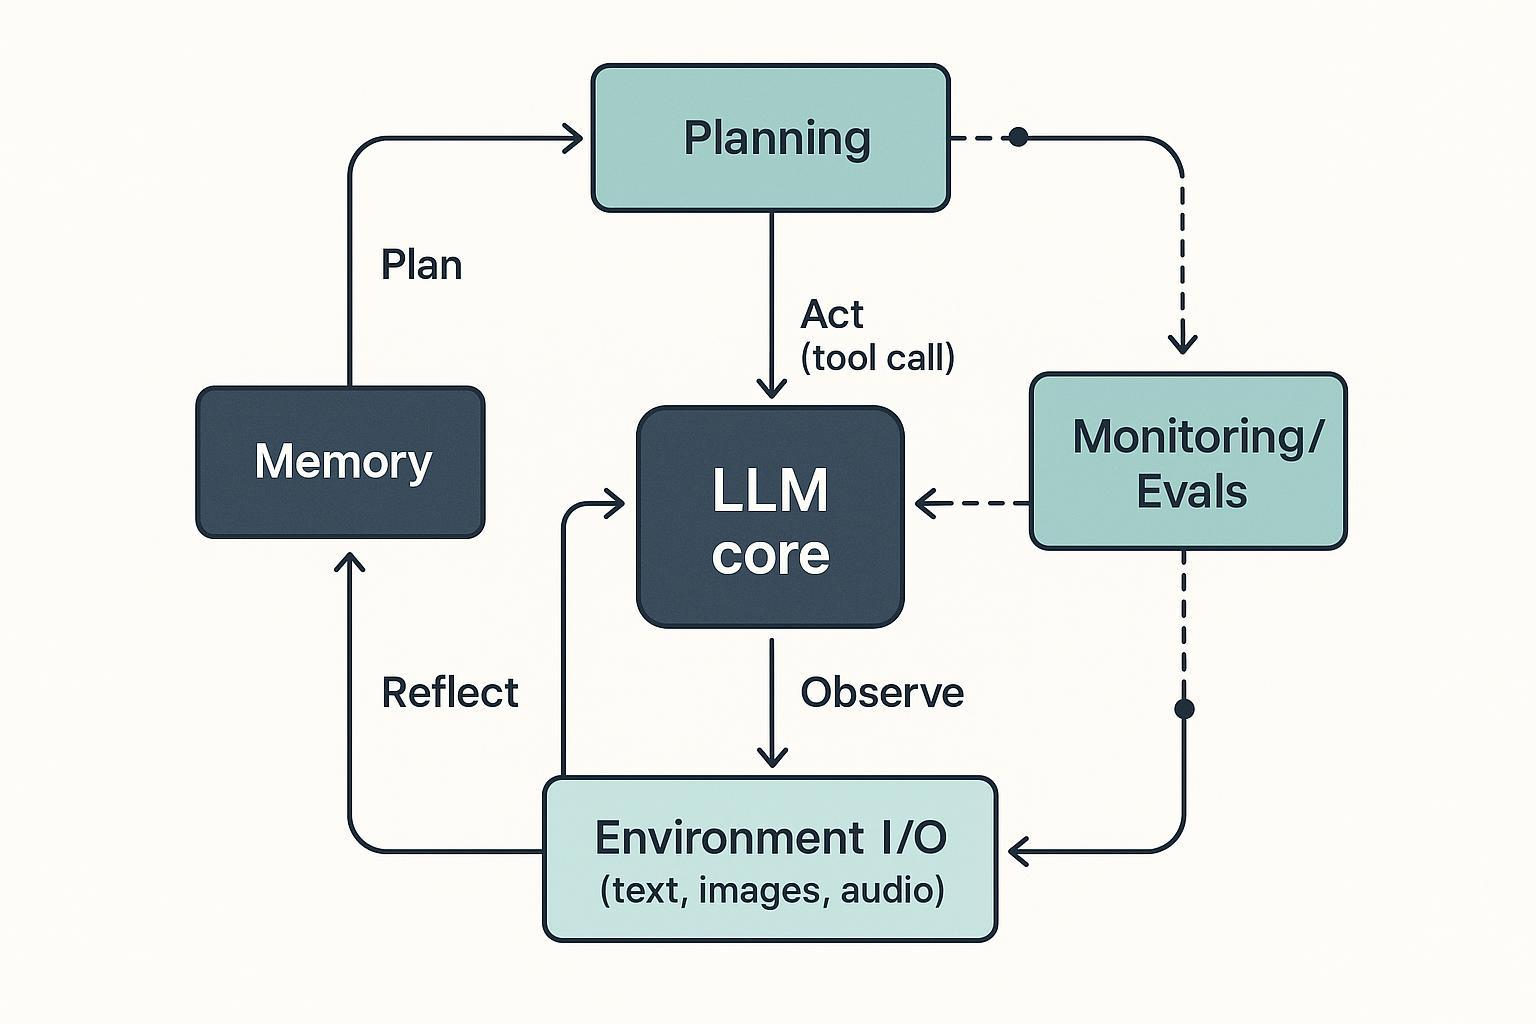
\includegraphics[width=0.75\textwidth]{images_pfe/concept Agent.jpg}
   \caption{Concept of AI Agents and Virtual Assistants.}
  \label{fig:concept_agent}
\end{figure}
\FloatBarrier

\vspace{0.2cm}

\noindent\textbf{Key Characteristics of Modern AI Agents:}

\vspace{0.2cm}

\noindent\textbf{(1) Natural Language Understanding:} Modern Agents are able to comprehend the verbal, written and also contextually-based utterances from a user in real-time. They would able to resolve and answer various queries such as to answer if I own X, to find Y, can you tell me something about Z, or can I do something on the PC.

\noindent\textbf{(2) Task Automation:} Represents complex sequences of actions, connect directly to different services (web applications, email client, local files, databases), or even simulate user activity on different applications without direct human interaction.

\noindent\textbf{(3) Contextual Awareness:} Effective agents ought to be able to manage their conversation context; this consists of keeping track of the history of the dialog, remembering facts about the world (a knowledge base), learning from past interactions and chasten their future behavior by making improvements.

\noindent\textbf{(4) Knowledge Integration:} Another crucial aspect of knowledge agent is its ability to aggregate data from a plurality of knowledge sources. So that knowledge agents are able to provide a comprehensive answer to queries posed by users.

\noindent\textbf{(5) Reasoning and Planning:} High end agents also know how to partition a task to several sub-tasks. Since, a task requested by the agent should be easily solvable by the robot. They will make an exhaustive search among possible ways to reach the objective. They are also able to reason about time constraints or material availability.

\FloatBarrier

% ═════════════════════════════════════════════════════════════════════════════
\section{\textcolor[HTML]{0066CC}{Large Language Models (LLMs)}}
\label{sec:llms}
% ═════════════════════════════════════════════════════════════════════════════

\subsection*{\textcolor[HTML]{003D99}{Overview and Core Architecture}}

All of the AI agents/virtual assistants that we have worked with are powered by a Large Language Model. An LLM is a type of deep neural network that has been trained on massive amounts of text data, such as book texts, websites, and other text sources. In LLM self-supervised learning, a model predicts continuations of a sequence of text, thereby allowing it to learn natural language patterns.
\begin{figure}[!htbp]
  \centering
  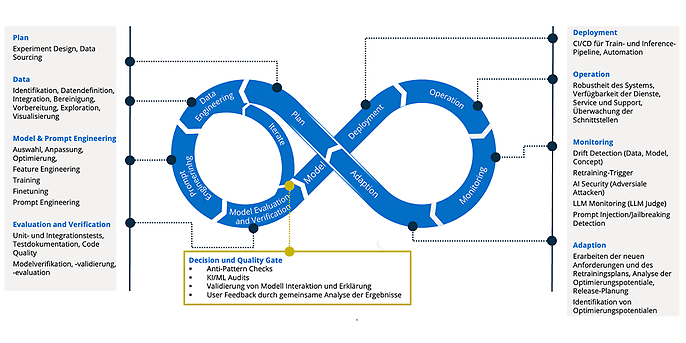
\includegraphics[width=0.75\textwidth]{images_pfe/LLM approach.png}
   \caption{Concept of Large Language Models (LLMs) and their architecture.}
  \label{fig:concept_llm}
\end{figure}
\FloatBarrier
\subsection*{\textcolor[HTML]{003D99}{Capabilities and Training Approaches}}

The task of these models is autoregressive language modeling, specifically the prediction of the next token in a sequence of text, given its previous tokens. The emergent capabilities that we see in the large-scale models are not directly encouraged by this training methodology, which is why the recent focus has been on instruction tuning (Fine-tuning large, pre-trained models on examples of following user instructions) and reinforcement learning from human preferences (RLHF) for the safer, more aligned and helpful models.

Because of the high flexibility of these systems, they can naturally be adapted to be foundation models that are particularly well-suited for an agent system, able to respond to a user's multifaceted queries whether as: a multi-turn conversational model; an instructed one, with clear reasoning why it came to a conclusion, or; prompted for structured data as output; and crucially, able to generalize between these tasks and adapt quickly to them with just small amounts of task specific fine-tuning via prompting techniques such as few shot learning.

\FloatBarrier

% ═════════════════════════════════════════════════════════════════════════════
\section{\textcolor[HTML]{0066CC}{Hallucination in Generative AI Systems}}
\label{sec:hallucination}
% ═════════════════════════════════════════════════════════════════════════════

\subsection*{\textcolor[HTML]{003D99}{Understanding Hallucination Phenomena}}

For LLM, given the enormous scale on which it's trained and its incredible skill, is capable of producing statements that are incredibly believable, but factually false. These falsehoods, known as hallucinations, occur for several possible reasons. In essence, hallucinatory responses arise as an accidental side effect of how these LLM's function. They don't remember pages from Wikipedia, instead they generate new text based on patterns of language that the model learned during its training phase. These patterns can cause an LLM to put together logical chains or claims, which are incorrect for the topic they're trained on.
\begin{figure}[!htbp]
  \centering
  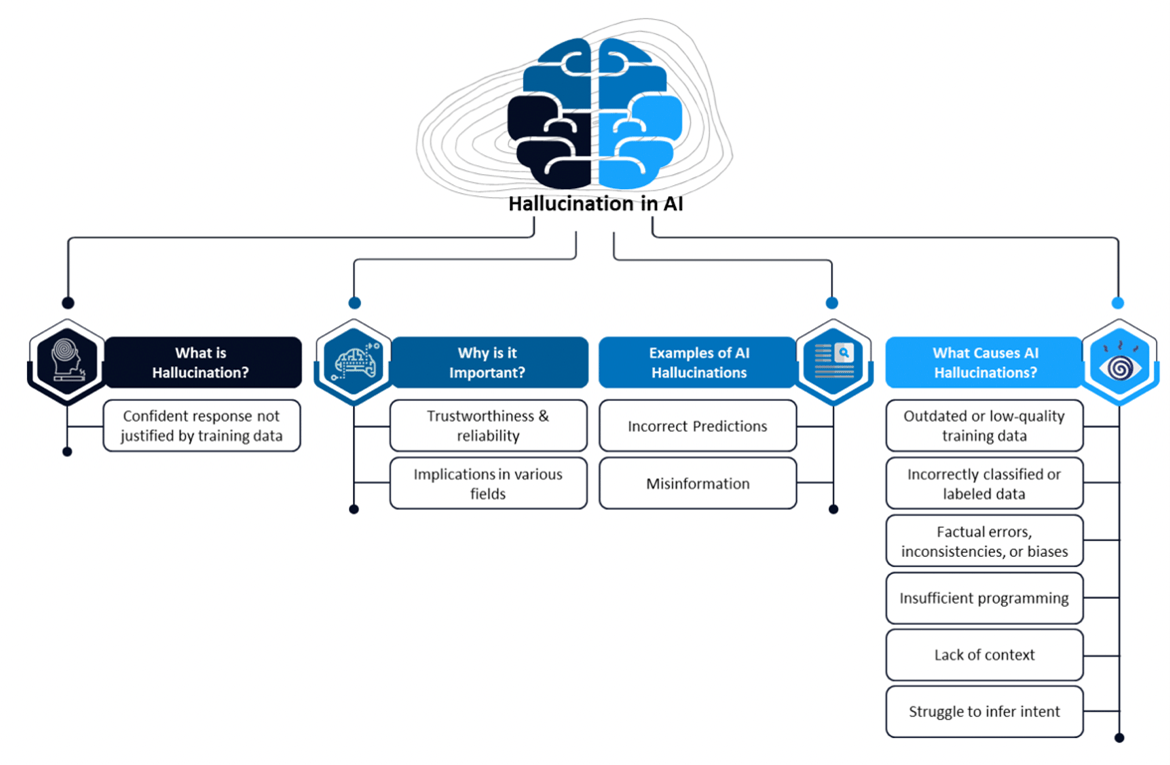
\includegraphics[width=0.75\textwidth]{images_pfe/AI hallucination.png}
   \caption{Concept of Hallucination in Generative AI Systems.}
  \label{fig:concept_hallucination}
\end{figure}
\FloatBarrier
\vspace{0.2cm}

\noindent\textbf{Sources and Types of Hallucination:}

\vspace{0.2cm}

\noindent\textbf{Factual Hallucination:} The model generates false facts that are inconsistent with any known factual knowledge.

\noindent\textbf{Logical Hallucination:} The model produces reasonable-looking reasoning chains that nonetheless contain logical fallacies or unwarranted assumptions.

\noindent\textbf{Context Hallucination:} Generating evidence for claims that are unsupported by, or are in contradiction to, the provided context. 

\noindent\textbf{Temporal Hallucination:} The model reported something that did not occur or who or what it reported is out of context using an incorrect time frame. 

\subsection*{\textcolor[HTML]{003D99}{Hallucination in Enterprise Applications}}

We posit that in the enterprise and governance applications in which LEON is applied, it is critical for the system to mitigate hallucination, especially in enterprise resource assignments, policy violations, invalid process recommendations, or wrong service invocation outcomes.

\FloatBarrier

% ══════════════════════Grounding and knowledge management ═══════════════════════════════════════════════════════
\section{\textcolor[HTML]{0066CC}{Grounding and Knowledge Management}}
\label{sec:grounding}
% ═════════════════════════════════════════════════════════════════════════════

\subsection*{\textcolor[HTML]{003D99}{Definition and Principles}}

\textbf{Grounding} refers to the process by which the outputs of an AI system are anchored, either textually, visually, or computationally, to sources of truth external to the system. The sources include various kinds of factual data, a writer's own documents, various kinds of current data, current systems, or trusted knowledge bases. With these components the agent is grounded and can be counted on to be traceable, accurate, and aware of the limits of its knowledge.

\vspace{0.2cm}

\noindent\textbf{Implementation Strategies for Grounding:}

\vspace{0.2cm}

\noindent\textbf{(1) Source Attribution:} The factual assertions made in an agent output should be traceable to either a source document, database, or API result.

\noindent\textbf{(2) Real-time Data Integration:} For a long lifespan agent, he can import much information from many authors. The agent may import that by its own or with the help of human.

\noindent\textbf{(3) Confidence Scoring:} Claims can be explicitly categorized as either passing through the system with high confidence, or inferred with a lower confidence.

\noindent\textbf{(4) Fallback Mechanisms:} If the agent is unsure about the current author or has not yet assigned an authority to the author, and if reliable authors are not the one the agent is currently addressing or would have addressed in his next step, fallback strategies must be used.

\FloatBarrier

% ═════════════════════════════════════════════════════════════════════════════
\section{\textcolor[HTML]{0066CC}{Retrieval-Augmented Generation (RAG)}}
\label{sec:rag}
% ═════════════════════════════════════════════════════════════════════════════

\subsection*{\textcolor[HTML]{003D99}{Framework and Architecture}}

\textbf{Retrieval-Augmented Generation (RAG)} is a powerful architectural pattern that attempts to fight hallucination and ground responses of LLMs by incorporating a Retrieval Component. The framework is straightforward; after receiving the user input, a Retriever extracts and returns a context document based on the query, and then the LLM uses thiscontext document and the query to produce an answer.
\begin{figure}[!htbp]
  \centering
  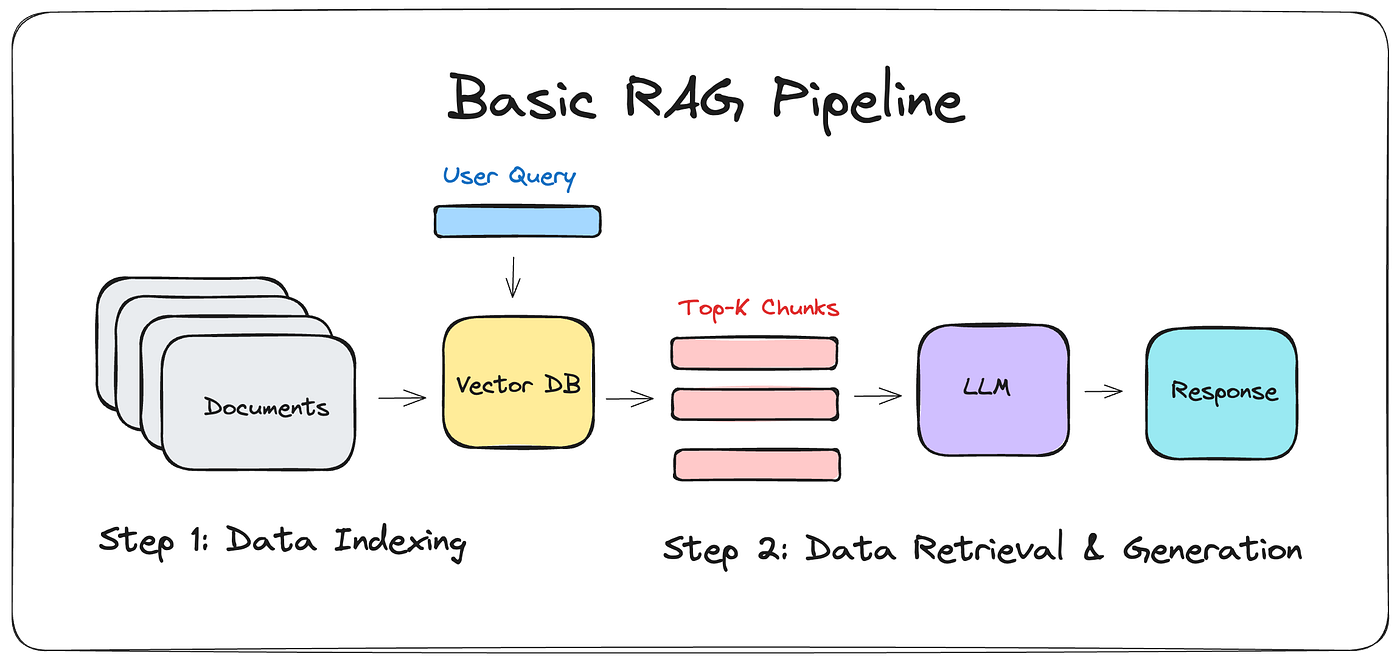
\includegraphics[width=0.75\textwidth]{images_pfe/RAG pipeline.png}
   \caption{Concept of Retrieval-Augmented Generation (RAG) pipeline.}
  \label{fig:concept_rag}
\end{figure}
\FloatBarrier
\vspace{0.2cm}

\noindent\textbf{RAG Architecture and Workflow:}

\vspace{0.2cm}

\noindent\textbf{(1) Query Encoding:} The step of taking the natural-language query input and turning it into a single number (called an embedding), such that all queries with the same semantic meaning are mapped to the same number.

\noindent\textbf{(2) Retrieval:} At retrieval, the user request is matched against a vector index of all the document/knowledge base entries, and content in contextually similar meaning is recovered.

\noindent\textbf{(3) Context Augmentation:} Factually relevant retrieved documents are directly concatenated to the front of the question text at inference time. The question itself remains in its original format, and no specific prompt formatting of context text is applied.

\noindent\textbf{(4) Grounded Generation:} The LLM generates a natural language answer to the query by conditioning on and grounding it within the retrieved context.

\noindent\textbf{(5) Source Citation:} A high quality RAG system must also provide accurate source citations. The system should have the ability to precisely identify all referential passages that contributed to the answer.

\subsection*{\textcolor[HTML]{003D99}{Key Advantages for Enterprise}}

\vspace{0.2cm}

\noindent\textbf{Accuracy and Hallucination Reduction:} RAG decreases inaccuracies and hallucinations by requiring the model to rely on provided resources rather than potentially spurious trends in the training data.

\noindent\textbf{Temporal Relevance:} This approach of dynamically pulling information makes them highly time-sensitive, enabling them to draw on up-to-date knowledge, as opposed to data collected at the time of training the LLM.

\noindent\textbf{Auditability and Compliance:} Each response returned would be easily traced and audited against sourced information. The responses will help satisfy enterprise governance, compliance and responsibility requirements.

\noindent\textbf{Knowledge Specialization:} While large language models are good general-purpose thinkers, they do not possess an organization's specific or domain specific knowledge. RAG alleviates the expense and difficulty of training a LLM on domain knowledge.

\noindent\textbf{Scalability:} LLMs are not able to grow with the scale of change in a business. The new knowledge can add to the index and LLMs do not need to be retrained.

Another significant aspect the agent needs, is the ability to use RAG for missioncritical operation. This may sound a bit dramatic for this case of study but this would be relevant in case of our governance agent, LEON. This is because in his case,  recommendations on how to use resources,  how to enforce a process or relevant technical document he refers to are based on external sources,  which he has to guarantee that he is actually taking the recommendations from these sources and not model hallucinations.

\FloatBarrier

% ═════════════════════════════════════════════════════════════════════════════
\section{\textcolor[HTML]{0066CC}{Orchestration: Conversation and Deterministic Automation}}
\label{sec:orchestration}
% ═════════════════════════════════════════════════════════════════════════════

\subsection*{\textcolor[HTML]{003D99}{Role in Enterprise AI Systems}}

\noindent\textbf{(1) Topic and Intent Classification:} The first step in orchestration is understanding what the user intends to accomplish. \textbf{Topics} represent broad functional areas (e.g., "resource allocation", "process compliance", "documentation validation"), while \textbf{intents} are specific actions within those domains (e.g., "who is available for task X", "check gate readiness", "validate specification"). Classification systems, often powered by LLMs or lightweight machine learning models, map user utterances to topics and intents, determining which automation workflow should be triggered.

\noindent\textbf{(2) Trigger Mechanisms:} A \textbf{trigger} is an event or condition that initiates an automated workflow. Triggers can be explicit (user-initiated via natural language: "Find team members qualified in embedded systems") or implicit (scheduled or event-driven: "Check all components' gate status daily"; "Notify when a specification update is posted"). Effective trigger design ensures that routine, repetitive tasks execute automatically while user-facing tasks respond immediately to requests.

\noindent\textbf{(3) Agent Workflows and Flows:} An \textbf{agent workflow} or \textbf{agent flow} is a structured sequence of deterministic steps that transform user intent into concrete outcomes. Unlike the probabilistic nature of LLM generation, workflows follow explicit branching logic, conditional rules, and predefined sequences. Workflows are composed of:

\vspace{0.1cm}


\noindent\indent • \textbf{Input Steps:} Retrieve user request parameters, context, and relevant domain information.

\noindent\indent • \textbf{Processing Steps:} Execute business logic—query databases, check compliance rules, validate constraints, apply transformations.

\noindent\indent • \textbf{Decision Points:} Branch based on conditions (if permission is granted, if availability exists, if specification is valid, etc.).

\noindent\indent • \textbf{Integration Steps:} Call external services, update systems, interact with APIs.

\noindent\indent • \textbf{Output Steps:} Format results, generate responses, provide citations and explanations.
\begin{figure}[!htbp]
  \centering
  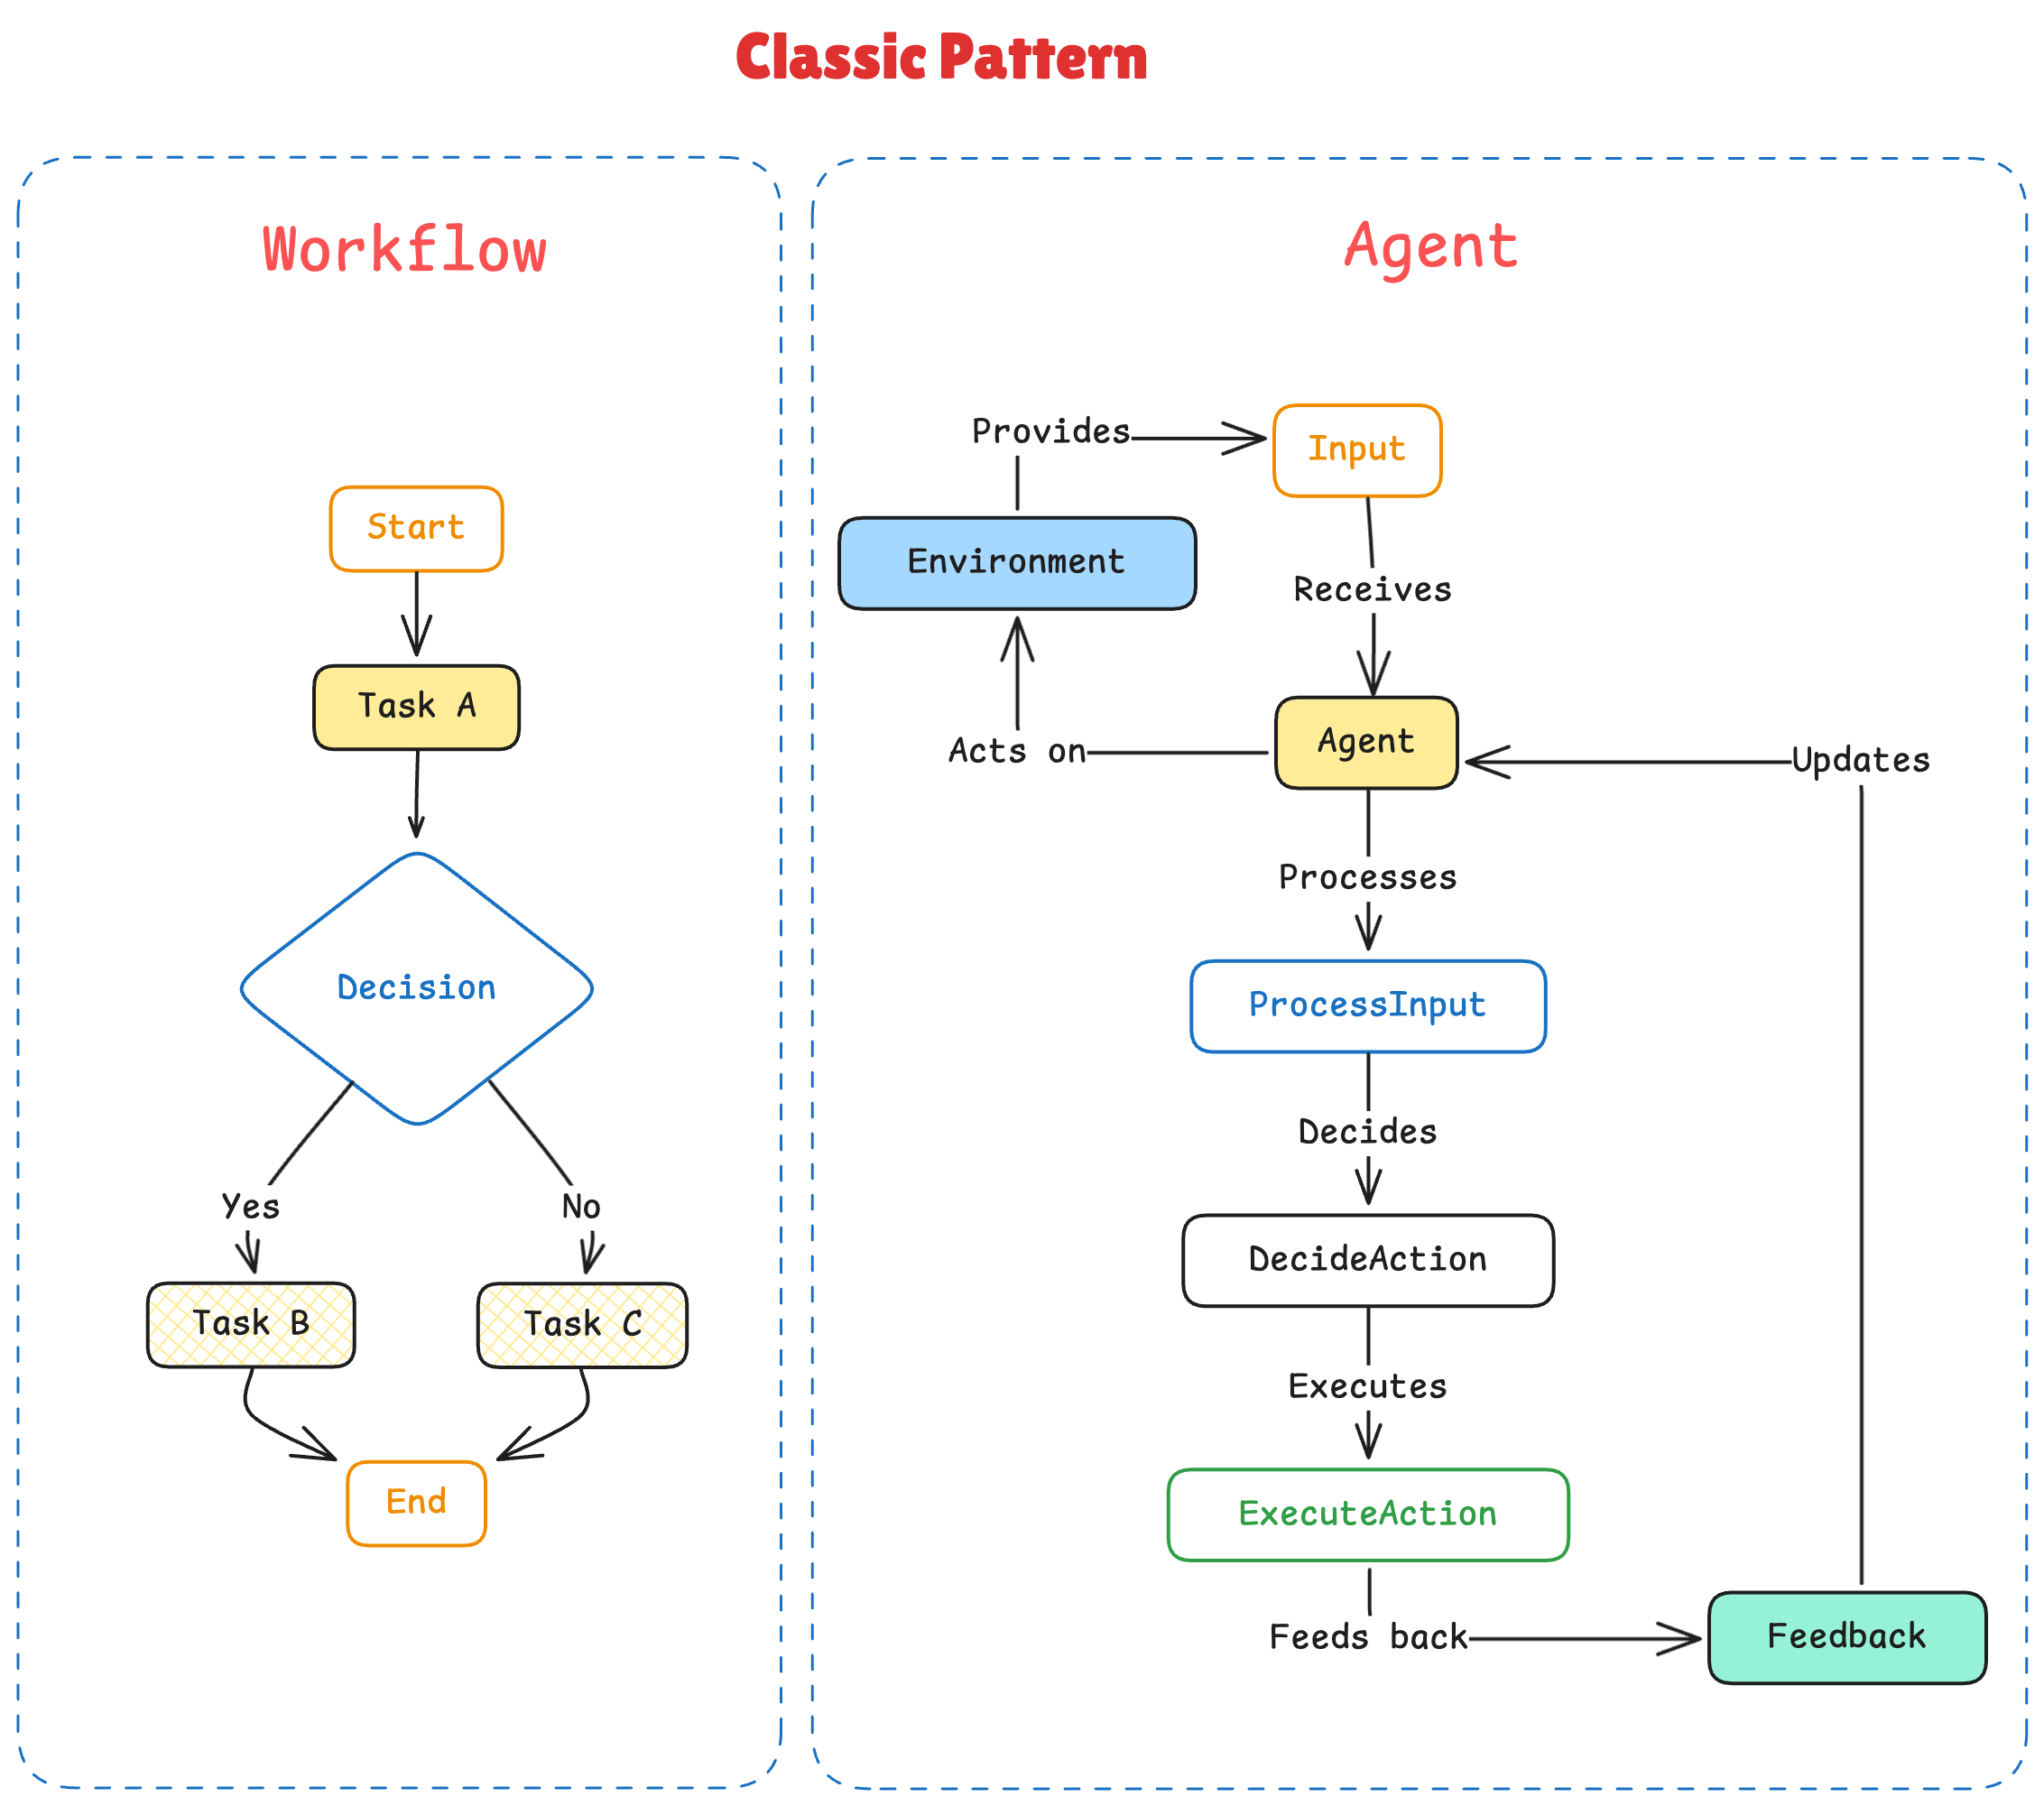
\includegraphics[width=0.75\textwidth]{images_pfe/agent workflow.png}
   \caption{Concept of Agent Workflows and Flows.}
  \label{fig:concept_agent_workflow}
\end{figure}
\FloatBarrier
\vspace{0.1cm}

\noindent\textbf{(4) API Connectors and Wrappers:} \textbf{API connectors} (or \textbf{wrappers}) are adapter modules that enable agent workflows to interact with external systems. A connector abstracts the complexity of underlying service APIs, providing a simplified interface for the agent. For example:

\vspace{0.1cm}

\noindent\indent • A \textbf{SharePoint connector} enables the agent to query document repositories, retrieve metadata, and check access permissions.

\noindent\indent • A \textbf{database connector} allows the agent to execute prepared queries against enterprise databases without exposing raw SQL or schema details.

\noindent\indent • A \textbf{email connector} enables the agent to compose and send messages on behalf of users, respecting approval workflows.

\noindent\indent • A \textbf{calendar connector} allows the agent to check availability, schedule meetings, and manage time-based events.

\vspace{0.1cm}

Connectors encapsulate error handling, authentication, rate limiting, and data transformation, providing the agent with reliable, safe interfaces to backend systems.

\subsection*{\textcolor[HTML]{003D99}{Power Automate and Repeatable Automation Logic}}

\vspace{0.2cm}

\textbf{Power Automate} (Microsoft's cloud-based workflow automation platform) exemplifies modern orchestration infrastructure. Power Automate "flows" are visual, low-code workflows that encode business logic in a format that is simultaneously human-readable (for business stakeholders) and machine-executable (for automation engines).
\begin{figure}[!htbp]
  \centering
  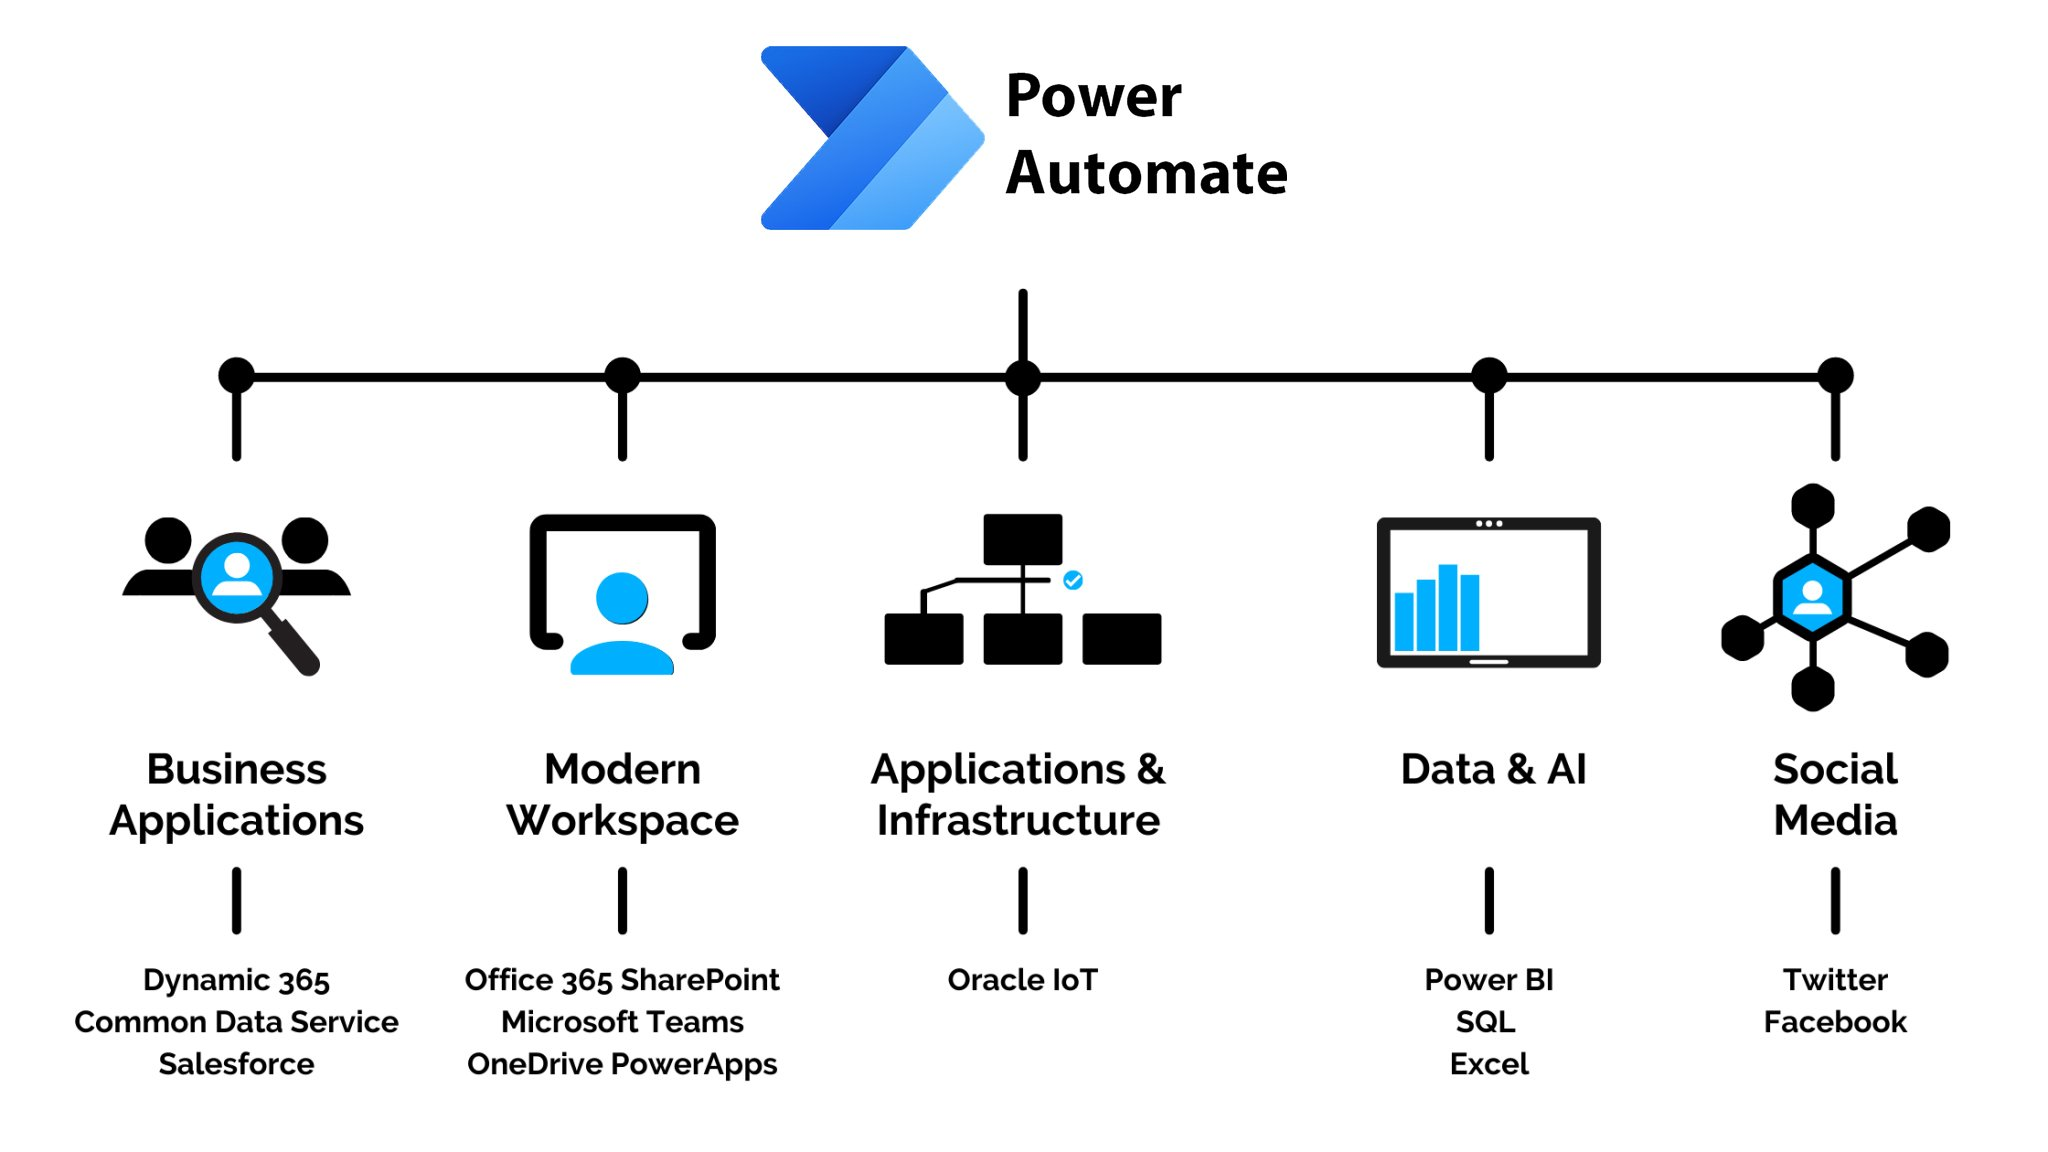
\includegraphics[width=0.75\textwidth]{images_pfe/power automate.jpg}
   \caption{Concept of Power Automate Flows.}
  \label{fig:concept_power_automate}
\end{figure}
\FloatBarrier
A Power Automate flow typically includes:

\vspace{0.2cm}

\noindent\textbf{Connectors:} Pre-built integrations with hundreds of enterprise systems (SharePoint, Exchange, SQL Server, Dynamics 365, Teams, Slack, Salesforce, etc.), eliminating the need to write custom integration code.

\noindent\textbf{Conditional Logic:} \texttt{If-Then-Else} branches, switch statements, and rule-based routing that make workflows deterministic and testable.

\noindent\textbf{Parallel Processing:} Simultaneous execution of independent steps (e.g., notify multiple stakeholders, check multiple systems) for efficiency.

\noindent\textbf{Approval Workflows:} Built-in approval steps that pause automation pending human review and decision, ensuring governance compliance.

\noindent\textbf{Data Transformation:} Tools for mapping, filtering, and transforming data between systems with different schemas or formats.

\noindent\textbf{Error Handling and Retry Logic:} Mechanisms to gracefully handle failures, retry failed steps, and notify administrators of issues.

\vspace{0.3cm}

By integrating LLM-based conversation with Power Automate flows, an agent becomes capable of both natural, flexible dialogue and reliable, repeatable automation. For instance:

\vspace{0.2cm}

\noindent\indent • User says: "Who is available to take the embedded software task for component X?" $\rightarrow$ Intent classified as "resource availability query" $\rightarrow$ Triggers a Power Automate flow that queries team database, checks calendars, filters by skill tags, and returns a ranked list grounded in authoritative sources.

\noindent\indent • User says: "Allocate Sarah to this task and notify the team" $\rightarrow$ Intent classified as "resource allocation" $\rightarrow$ Triggers an approval flow if required, updates the project management system, sends notifications via email/Teams, and logs the action for audit.

\noindent\indent • Scheduled trigger fires daily: Check all components' gate maturity status $\rightarrow$ Automatically queries engineering database, retrieves gate status from SharePoint portal, identifies components at risk of schedule slippage, and generates a summary report for governance meetings.

\subsection*{\textcolor[HTML]{003D99}{Orchestration in the Context of LEON}}

\vspace{0.2cm}

For the \textbf{LEON} governance agent, orchestration is essential to operationalize the agent's capabilities. Rather than relying solely on LLM outputs (which may hallucinate or miss domain constraints), LEON's workflows embed governance rules, access control policies, compliance checks, and approval gates. Conversations with LEON feel natural ("Who owns the electrical systems for the 3008?"), but behind the scenes, deterministic orchestration ensures accuracy (querying the authoritative organization database, checking user permissions, verifying data currency) and traceability (logging the query, the retrieved data sources, the response, and the timestamp).

This orchestration-driven approach transforms LEON from a conversational interface into a \textbf{trustworthy governance assistant}\textemdash one where accuracy is primarily achieved through system integration and rule enforcement rather than relying on the agent to "remember" domain knowledge or reason about complex policies.

% ═════════════════════════════════════════════════════════════════════════════
% End of Chapter 3: État de l'Art et Fondations Techniques
% ═════════════════════════════════════════════════════════════════════════════
